\section{Limited-Memory BFGS Method}\label{sec:QNM}
The conjugate gradient has led us to nice properties and faster convergence than the classic gradient descent method. Another interesting class of optimization algorithms are the quasi-Netwon methods, they are characterized by further interesting convergence properties such as superlinear convergence.

The first quasi-Newton method was developed by W. C. Davidon in 1959 \cite{davidon}, and, like steepest descent, only the gradient must be provided at each iteration \cite{Nocedal} and, moreover, allows to avoid the direct computation of the hessian, not feasible to compute in some problem and required in the newton method. By measuring the changes in gradients, it construct a model of the objective function that is good enough to produce superlinear convergence. In 1963 Fletcher and Powell \cite{10.1093/comjnl/6.2.163} have demonstrated theoretically and with numerical examples that it was considerably superior to other previously methods available at that time - It transformed the nonlinear optimization. In fact, the improvement over steepest descent was dramatic and this is the reason why, over the years, several variants of this method were proposed to achieve even better results in the nonlinear optimization. The most popular quasi-Newton algorithm is the Broyden–Fletcher–Goldfarb–Shanno (BFGS) method but even if it solves the problem the hessian calculation by replacing it with an approximation, the BFGS can be only used in unconstrained optimization problem where the number of variables allow to keep computational cost and storage feasible. \cac{qui volevo fare una piccola intro a BFGS come sta fatta a pagina 177, magari spiega meglio la roba anche a formule}In fact, the hessian approximations generated by the quasi-Newton, as BFGS, are usually dense, even when the true Hessian is sparse, and with $n$ variables it require $O(n^2)$ in storage complexity. Many applications raise unconstrained optimization problems with thousands or millions of variables, as in a neural network model, and those approch become unfeasible to use.

Since our objective function lies in the case of large scale optimization problem, here will take in analysis the study of a limited memory quasi-Newton method for large scale optimization, useful when hessian matrices cannot be computed at a reasonable cost or are not sparse (respectively problems occurred in Newton and quasi-Netwon methods), known as the \emph{limited-memory BFGS} (L-BFGS). The hessian approximations that can be stored compactly by using just a few vectors of length $n$ allowing the user to control the amount of storage required by the algorithm. 
\newline\cac{L'introduzione al capitlo è finita, vanno dette queste cose. Non so dove, qui o sparse durante la trattazione\begin{itemize}
    \item è facile dimostrare praticamente le proprietà di super convergenza in bfgs e l-bfgs
    \item problema aperto realtivo alla convergenza globale, quindi noi andremo ad analizzare sotto quali considerazioni abbiamo la super convergenza nel caso non lineare
\end{itemize}}\\
\subsection{Limited-Memory BFGS}
\cac{sarà il caso di aprire una nuova sottosezione per l'algoritmo o bho}\\
\cgv{Forse mi piace più senza sottosezione, come per il conjugate.}\\
This method can be seen as extensions of the conjugate gradient method seen in Sec. \ref{sec:NCG}, in which additional storage is used to accelerate convergence. The L-BFGS is based on the following updating formula:
\begin{equation}
    \mathbf{w}_{k+1}=\mathbf{w}_k + \alpha_k \, \mathbf{d}_k,
    \label{eq:bfgs_update}
\end{equation}
where $\alpha_k$ is the step lenght, and $\mathbf{d}_k$ is the search direction. The complete method is described by Algo. \ref{alg:bfgs}.

\begin{algorithm}[H]
\label{alg:bfgs}
\SetAlgoLined
 \textbf{init}: $\mathbf{w}_0$ with some small random values, $max\_iter$, $m  > 0$\;
 $k \leftarrow 0$\;
 \While{k < max\_iter}{
  Choose the initial matrix $\mathbf{H}_k^0$ by using
  \begin{equation}\label{initial_matrix}
      \mathbf{H}_k^0 = \gamma_k \, \mathbf{I} = \frac{\mathbf{s}_{k-1}^\mathsf{T} \mathbf{y}_{k-1}}{\mathbf{y}_{k-1}^\mathsf{T}\mathbf{y}_{k-1}} \,\mathbf{I}
  \end{equation}\;
  Compute the search direction $\textbf{d}_k \leftarrow -\mathbf{H}_k \, \mathbf{g}_k$ from Algo. \ref{alg:bfgs_loop}\;
  Compute the learning rate $\alpha_k$ with a Line Search satisfying the Strong Wolfe conditions (always try $\alpha_k = 1$ first)\;
  Update the weights $\mathbf{w}_{k+1} \leftarrow \mathbf{w}_k + \alpha_k \mathbf{d}_k$\;
  \If{$k > m$}{
  Discard the oldest vector pair $\{ \mathbf{s}_{k-m}, \, \mathbf{y}_{k-m}\}$ from storage\;}
  Compute and save $\mathbf{s}_k \leftarrow \mathbf{w}_{k+1} - \mathbf{w}_k$, $\mathbf{y}_k = \mathbf{g}_{k+1} - \mathbf{g}_k$\;
  Set $k \leftarrow k + 1$\;
 }
 \caption{L-BFGS}
\end{algorithm}
\vspace{+6pt}

\noindent Equation (\ref{initial_matrix}) describes an efficient method for choosing the initial matrix $\mathbf{H}_k^0$, where $\gamma_k$ is the scaling factor that attempts to estimate the size of the true Hessian matrix along the most recent search direction (allowing $\mathbf{H}_k^0$ to vary between iterations). This choice helps to ensure that the search direction $\mathbf{d}_k$ is well scaled, and as a result the step length $\alpha_k = 1$ is accepted in most iterations.\\
\cgv{Nelle prime $m-1$ iterazioni, L-BFGS è uguale a BFGS, se la matrice iniziale è la stessa. Quindi deduco che i criteri di convergenza, quantomeno nelle prime $m-1$ iterazioni, siano uguali. Dagli esperimenti fatti, è stato visto che $3 \leq m \leq 20$ permette di ottenere buoni risultati.}

\subsection{Search Direction}\label{search_direction_qn} 
\cgv{rho, s ed y scritti in grassetto. Controllare se corretto.}\\
The search direction at the k-th iteration is defined by
\begin{equation}
    \mathbf{d}_k = - \mathbf{H}_k \, \mathbf{g}_k,
\end{equation}
where $\mathbf{H}_k$ is a \emph{modified} version of the inverse Hessian approximation, which is updated at every iteration by formula
\begin{equation}
    \mathbf{H}_{k+1}=\mathbf{V}_k^\mathsf{T} \, \mathbf{H}_k \, \mathbf{V}_k + \boldsymbol\rho_k \, \mathbf{s}_k \, \mathbf{s}_k^\mathsf{T},
    \label{eq:bfgs_H_update}
\end{equation}
where 
\begin{equation}
    \boldsymbol\rho_k = \frac{1}{\mathbf{y}_k^\mathsf{T} \, \mathbf{s}_k}, \,\,\,\,\,\,\,\, \mathbf{V}_k = \mathbf{I} \, - \, \boldsymbol\rho_k \, \mathbf{y}_k \, \mathbf{s}_k^\mathsf{T},
    \label{}
\end{equation}
and
\begin{equation}
    \mathbf{s}_k = \mathbf{w}_{k+1} - \mathbf{w}_k, \,\,\,\,\,\,\,\, \mathbf{y}_k = \mathbf{g}_{k+1} - \mathbf{g}_k.
    \label{}
\end{equation}
Since the $\mathbf{H}_k$ of quasi-Newton methods is generally a dense matrix, storing and manipulating it is prohibitive when we will approach large problems. To overcome this issue, a certain number ($m$) of vector pairs $\{ \mathbf{s}_i, \, \mathbf{y}_i\}$ are stored, to obtain an implicitly modified version of $\mathbf{H}_k$. The product $\mathbf{H}_k \, \mathbf{g}_k$ can be obtained by Algo. \ref{alg:bfgs_loop}.

\begin{algorithm}[H]
\label{alg:bfgs_loop}
\SetAlgoLined
 $\mathbf{q} \leftarrow \mathbf{g}_k$ \;
 \For{$i = k-1, \,\, k-2, \,\, ... \,\, , \,\, k-m$}
    {$\boldsymbol\alpha_i \leftarrow \boldsymbol\rho_i \, \mathbf{s}_i^\mathsf{T} \, \mathbf{q}$\;
    $\mathbf{q} \leftarrow \mathbf{q} - \boldsymbol\alpha_i \, \mathbf{y}_i$\;} 
 \EndFor
 $\mathbf{r} \leftarrow \mathbf{H}_k^0 \, \mathbf{q}$\;
 \For{$i = k-m, \,\, k-m+1, \,\, ... \,\, , \,\, k-1$}
    {$\boldsymbol\beta \leftarrow \boldsymbol\rho_i \, \mathbf{y}_i^\mathsf{T} \mathbf{r} $\;
    $\mathbf{r} \leftarrow \mathbf{r} + \mathbf{s}_i(\boldsymbol\alpha_i - \boldsymbol\beta)$\;} 
 \EndFor
 \textbf{return} $\mathbf{H}_k \, \mathbf{g}_k = \mathbf{r}$
 \caption{L-BFGS two-loop recursion}
\end{algorithm}
\cgv{Spiegare meglio come fa ad essere positive-definite? (lo è). Vedi pag. 141}\\
To ensure that $\mathbf{d}_k$ will be a \emph{descent direction}, $\mathbf{H}_{k+1}$ must be \emph{positive-definite}. As shown in \cite{Nocedal}, this holds when the initial approximation $\mathbf{H}_{0}$ is positive definite and the \emph{curvature condition} $\mathbf{s}_k^\mathsf{T}\mathbf{y}_k > 0$ is verified. When dealing with non-convex functions, the curvature condition will be guaranteed if the line search, which chooses the step length $\alpha_k$, satisfies the strong Wolfe conditions.\\
\cgv{\textbf{Scrivere da qualche parte una cosa di questo tipo}: During the first $m$ iterations the method is identical to the BFGS method. For $k>m$ $\mathbf{H}_k$ is obtained by applying $m$ BFGS updates to $\mathbf{H}_0$ using information from the $m$ previous iterations.}

\subsection{Step-length}\label{alpha_qn}
As noted above, a line search satisfying the \emph{strong Wolfe conditions}, with $0 \leq c_1 \leq c_2 \leq 1$, has to be performed to find the right step length $\alpha_k > 0$. The procedure, described in \ref{alpha}, is the same used for the conjugate gradient method. However, in this case, the constant $c_2$ is equal to 0.9 and, step $\alpha_0 = 1$ should always be used as the initial trial step length \cgv{Se va bene abbiamo la superlinearità (?)}. Moreover, the satisfaction of strong Wolfe conditions makes L-BFGS updating stable.

\subsection{Superlinear convergence}\label{global_convergence_qn}
\cgv{Secondo me l'analisi dei ragazzi di padova è sbagliata. Dobbiamo stare attenti a cosa dire, perché a pag. 153 dice che il BFGS con converge globalmente per le funzioni con convesse (però forse, con strong wolfe riusciamo? non è chiaro dal libro)}\cac{concordo, appena ci sei se ne parla}\\
For the purposes of this section, we make the following assumptions on the objective function.
\begin{assumption}
\label{as:3}
The objective function is twice continuously differentiable. 
\end{assumption}
\begin{assumption}
\label{as:4}
$\mathbf{H}_k$ need is positive definite.
\end{assumption}
\cgv{Spiegare perché le due assunzioni sono verificate.}\\

\cgv{Theorem 3.6 a pag.46}
\begin{theorem}
\label{th:superlinearl_qn}
Suppose $L$ is twice continuously differentiable. Consider the iteration $\mathbf{w}_{k+1}=\mathbf{w}_k + \alpha_k \mathbf{d}_k$, where $\mathbf{d}_k$ is a descent direction and $\alpha_k$ satisfies the strong Wolfe conditions with $c_1 \leq \frac{1}{2}$. If the sequence $\{ \mathbf{w}_k\}$ converges to a point $\mathbf{w^*}$ such that $\nabla L (\mathbf{w}^*) = 0$ and $\nabla^2 L(\mathbf{w}^*)$ is positive definite, and i the search direction satisfies
\begin{equation}
      \lim_{k\to\infty} \frac{\| \nabla L_k - \nabla^2 L_k \, \mathbf{d}_k\|}{\| \mathbf{d}_k\|} = 0,
\end{equation}
then
\begin{itemize}
    \item the step length $\alpha_k = 1$ is admissible for all $k>k_0$; and
    \item if $\alpha_k = 1$ for all $k>k_0$, $\{ \mathbf{w}_k\}$ converges to $\mathbf{w}^*$ superlinearly. 
\end{itemize}
\end{theorem}
\cgv{Allineare}\\
Since $\mathbf{d}_k$ is a quasi-Newton search direction in the form of $\mathbf{d}_k = - \mathbf{B}_k^{-1} \, \mathbf{g}_k$, then (27) is equivalent to
\begin{equation}
      \lim_{k\to\infty} \frac{\| (\mathbf{B}_k - \nabla^2 L(\mathbf{w}^*) \, \mathbf{d}_k) \mathbf{d}_k\|}{\| \mathbf{d}_k\|} = 0.
\end{equation}
Therefore, is sufficient that the $\mathbf{B}_k$ become increasingly accurate approximations to $\nabla^2 L(\mathbf{w}^*)$ along the search direction $\mathbf{d}_k$ to guarantee the superlinear convergence rate.

\cgv{Theorem 3.7 a pag.47}
\begin{theorem}
\label{th:superlinearl_qn}
Suppose $L$ is twice continuously differentiable. Consider the iteration $\mathbf{w}_{k+1}=\mathbf{w}_k + \mathbf{d}_k$ (that is, the step length $\alpha_k$ is uniformly 1) and that $\mathbf{d}_k$ is given by $\mathbf{d}_k = - \mathbf{B}_k^{-1} \, \mathbf{g}_k$. Let us assume also that $\{ \mathbf{w}_k\}$ converges to a point $\mathbf{w^*}$ such that $\nabla L (\mathbf{w}^*) = 0$ and $\nabla^2 L(\mathbf{w}^*)$ is positive definite. Then $\{ \mathbf{w}_k\}$ converges superlinearly if and only if (28) holds.
\end{theorem}

\cgv{Theorem 6.5 a pag.154-155-156}
\begin{theorem}
\label{th:superlinearl_convex}
Let $\mathbf{B}_0$ be any symmetric positive definite initial matrix, and let $\mathbf{w}_0$ be a starting point for which Assumption \ref{as:3} and Assumption \ref{as:4} are satisfied. Then the sequence $\mathbf{w}_k$ generated by Algorithm \ref{alg:bfgs} converges to the minimizer $\mathbf{w^*}$ of $L$.
\end{theorem}

Theorem \ref{th:superlinearl_convex} shows that the rate of convergence of the iterates is linear. In particular, the sequence $\| \mathbf{w}_k - \mathbf{w_0}\|$ converges to zero rapidly enough that 
\begin{equation}\label{eq:seq_to_zero_rapidly}
    \sum_{k=1}^{\infty} \| \mathbf{w}_k - \mathbf{w_0}\| < \infty.
\end{equation}

\cgv{Assumption 6.2 a pag.156}
\begin{assumption}
\label{as:5}
The Hessian matrix $G$ is Lipschitz continuous at $x^*$, that is,
\begin{equation}\label{eq:hessian_Lcontinuity}
    \| G(x) - G(x^*) \| \leq L\,\|x - x^*\|,
\end{equation}
for all x near x^*, where L is a positive constant.
\end{assumption}

\cgv{Theorem 6.6 a pag.158}
\begin{theorem}
\label{th:superlinearl_nonconvex}
Suppose that $L$ is twice continuously differentiable and that the iterates generated by BFGS algorithm converge to a minimizer $\mathbf{w^*}$ at which Assumption \ref{as:5} holds. Suppose also that (\ref{eq:seq_to_zero_rapidly}) holds. Then $\mathbf{w}_k$ converges to $\mathbf{w^*}$ at a superlinear rate.
\end{theorem}

\cgv{Inserire le cose che servono per garantire la superlinearità nei casi non convessi.}\\
\cgv{Per la convergenza globale, per ora non aggiungerei altro, visto che non sono certa che si posa dimostrare.}\\
\cgv{Riprendo a lavorare verso le 16:40/17:00}

\documentclass[11pt]{article}
%\usepackage[margin=1in]{geometry} 
\usepackage{template}

        

\usepackage[utf8]{inputenc} % allow utf-8 input
\usepackage[T1]{fontenc}    % use 8-bit T1 fonts
\usepackage{hyperref}       % hyperlinks
\usepackage{url}            % simple URL typesetting
\usepackage{booktabs}       % professional-quality tables
\usepackage{amsfonts}       % blackboard math symbols
\usepackage{nicefrac}       % compact symbols for 1/2, etc.
\usepackage{microtype}      % microtypography
\usepackage{lipsum}
\usepackage[labelfont=bf]{caption}
\usepackage{subcaption}
\usepackage{amsmath,amsthm,amssymb}
\usepackage[english]{babel}
\usepackage{comment}
\usepackage{enumitem}
\usepackage[ruled,vlined]{algorithm2e}
\usepackage{algorithmic}
%\usepackage{algorithmicx}

\usepackage{graphicx}
\graphicspath{ {images/} }

\usepackage{floatrow}
\usepackage{listings}
\usepackage{minted}
\floatsetup[listing]{style=Plaintop}  

\usepackage{amsmath}               
  {
      \theoremstyle{plain}
      \newtheorem{assumption}{Assumption}
  }
  
\newtheorem{theorem}{Theorem}
\newtheorem{corollary}{Corollary}

\usepackage{float}
\usepackage{texments}
\usestyle{default} %other useful styles are, bw,  borland, vs
\usepackage[dvipsnames]{xcolor}
\usepackage[toc,page]{appendix}
%\usepackage[titletoc]{appendix}
\usepackage{minted}

\usepackage{chngcntr}
\counterwithin{figure}{section}
\counterwithin{table}{section}

%citation
\usepackage{epigraph}

\usepackage{graphicx}

\newcommand{\norm}[1]{\left\lVert#1\right\rVert}

\newcommand{\cac}[1]{{\textcolor{blue}[\textcolor{blue}{\bf{AC: }}{ \textcolor{blue}
              {#1}]}}}
\newcommand{\cgv}[1]{{\textcolor{RedOrange}[\textcolor{RedOrange}{\bf{GV: }}{ \textcolor{RedOrange}
              {#1}]}}}

%\setcitestyle{square}

%%%%%%%%%%%%%%%%%%%%%%%%%%%%%%%%
%%      Tittle Page Start     %%
%%%%%%%%%%%%%%%%%%%%%%%%%%%%%%%%
\title{training a neural network with conjugate gradient and limited-memory bfgs methods}
\author{
  Alessandro Cudazzo \\
  \texttt{alessandro@cudazzo.com} \\
  %% examples of more authors
   \And
  Giulia Volpi \\
  \texttt{giuliavolpi25.93@gmail.com} \\
  \AND
  Department of Computer Science, University of Pisa, Pisa, Italy
  %% Coauthor \\
  %% Affiliation \\
  %% Address \\
  %% \texttt{email} \\
  %% \And
  %% Coauthor \\
  %% Affiliation \\
  %% Address \\
  %% \texttt{email} \\
  %% \And
  %% Coauthor \\
  %% Affiliation \\
  %% Address \\
  %% \texttt{email} \\
}

%%%%%%%%%%%%%%%%%%%%%%%%%%%%%%%%
%%       Tittle Page End      %%
%%%%%%%%%%%%%%%%%%%%%%%%%%%%%%%%

\begin{document}

\maketitle
\begin{abstract}
Neural Networks are highly expressive models that have achieved the state of the art performance in many tasks as pattern recognition or natural language processing. Usually, stochastic momentum methods coupled with the classical Backpropagation algorithm for the gradient computation is used in training a neural network.
In recent years several methods have been developed to accelerate the learning convergence of first-order methods such as \textit{Classic Momentum}, also known as \textit{Polyak's heavy ball method} \cite{Polyak1964}, or the \textit{Nesterov} momentum \cite{10029946121}.
This work aims to go beyond the first-order methods and analyse some variants of the conjugate gradient (CG) and a specific case of limited-memory quasi-Newton class called L-BFGS as optimization methods to accelerate the learning processes of a feedforward neural network by combined them with the use of a line search that respects the Frank-Wolfe conditions. 
\end{abstract}

\section{Introduction}


Over the years neural networks (NN) have been widely used in many areas, such as pattern recognition or image segmentation where they have overcome classic computer vision algorithms with the use of Convolution Neural Networks (CNN) \cite{DBLP:journals/corr/BadrinarayananK15} and very quickly became the state of the art in many other areas ( i.e. speech recognition, natural language processing, audio recognition all well illustrated in \cite{Goodfellow-et-al-2016}). 
As defined in \cite{Mitchell97}, a NN, as any other machine learning (ML) models, is said to learn from experience to some class of tasks if the performance, measured by a metric, improves with that experience.
Usually, the learning process that allows the improvement of the performance is related to an optimization algorithm where a quantity, called Error, is minimized/maximized: this is why the field of optimization is so central in machine learning. The optimization process can concern both the area of constrained optimization (i.e. in Support Vector Machine) or unconstrained (i.e in NN) and we will focus on the last one. With respect to neural networks and unconstrained optimization, the stochastic gradient descent (SGD) coupled with the back-propagation (BP) algorithms, for the gradient computation, remains a popular supervised learning algorithm to train a NN but is not the fastest in terms of convergence. 
The SGD is a first-order method and the convergence can be improved through the use of acceleration methods that are already well known in the classical literature of unconstrained optimization: \textit{Classic Momentum} also known as \textit{Polyak's heavy ball method} \cite{Polyak1964} or the \textit{Nesterov} momentum \cite{10029946121} developed respectively in 1960 e 1983. In \cite{sutskever2013} has been proved that the last two methods are very efficient in performing the training of a neural network without the use of second-order optimization methods. With this work, we want to go further beyond the classical first-order methods and investigate more complex methods that use high-order information during the training phase such as Nonlinear Conjugate Gradient and the L-BFGS from the class of Limited-Memory Quasi-Newton. Those methods lead to  a more accurate choice of the search direction and of the step size, by using information
from the second-order approximation. Even better, L-BFGS achieves super-linear convergence.

The remaining text is structured as follows. In Section~\ref{sec:NN}, we have summarised all the assumptions for neural networks seen as an unconstrained optimization problem. In section \ref{sec:NCG} and \ref{sec:QNM} the conjugate gradient and the limited-memory BFGS methods will be illustrated. The experiments are shown in Section~\ref{sec:experiment}, Subsections~\ref{sec:monks} and \ref{sec:cup} respectively contain the results of MONK and CUP, while Section~\ref{sec:conclusions} is devoted to conclusions.



\section{The Neural Network}
\label{sec:NN}
The design of a Neural Networks model is biologically inspired by the brain and it's offer properties and capabilities \cite{Mitchell97,Goodfellow-et-al-2016, haykin2009neural}. This machine learning model has an elastic and adaptive ability, capable of learning from experience (the data provided) through a supervised process.  It can be considered as a network of interconnected units (artificial neurons) that adapt to perform a given task with the ability also to discover new knowledge. It can solve either a classification (binary/multi-class) or regression tasks. In this work, we will analyze a neural network from a mathematical point of view and a NN can be seen as a flexible function $h(\mathbf{x})$ that is a nested non-linear function:
\begin{equation}
    \label{eq:nn_function}
    h(\mathbf{x}) = f_k \left( \sum_{j}^J w_{kj} f_j \left( \sum_{i}^I w_{ji}x_i \right)\right) %= f_k \left( \sum_{j}^M w_{kj} f_j \left( net_j \right)\right) = f_k \left(net_k\right)
\end{equation}
where $h(\mathbf{x})$ is relative to a NN with one output neuron on the output layer, one hidden layer with J hidden neurons and input $\mathbf{x} \in \mathbb{R}^I$. Where $f_k$ is the activation function output neuron (linear or nonlinear function), $w_{kj}$ is a specific wights of the output neuron connected to the $j$-th hidden output neuron $f_j$ (a nonlinear activation function) that takes as input the linear combination of the products between $w_{ji}*x_i$.

So, the most important components of a NN are the nodes and architecture. Each node in the network will have associated a number of weights equal to the input of that node, a bias (which in our work will be included in the weights vector) and an activation function. The network can have different architectures with one or more hidden layers but the important thing is that each node in the hidden layers has a non-linear activation function (e.g. sigmoid). This allows the neural network to implement a linear basic expansion that is flexible and adaptive during the learning process thought the free parameters ($\mathbf{w}$) inside the non-linear activation function. Moreover, different architectures can lead to different hypothesis spaces that make the network more or less expressive for the task we are solving. This characterizes the neural networks by an important result which is the universal approximation theorem: an MLP network can approximate (arbitrarily well) every input-output mapping (provided enough units in the hidden layers). As concerns, the activation functions of neurons in the output layer can be either linear in case of a regression task or non-linear (e.g. sigmoid, softmax) in case of binary or multiclass classification tasks.

As in any other ML framework, we need a \emph{learning algorithm} that allows adapting the free-parameters of the model based on data provided in order to obtain the best approximation of the target function. This is often realized in terms of minimization of an error function on the training data set:
\begin{equation}
    \mathbf{w}^* = \min_{\mathbf{w} \;	\in \; \mathbb{R}^n} E(\mathbf{w})
\end{equation}
given a set of $l$ training examples $(\mathbf{x}_p,\mathbf{d}_p)$, where $\mathbf{x}_p \in \mathbb{R}^I$ and $\mathbf{d}_p \in \mathbb{R}^R$ we want to find the weights vector $\mathbf{w}^* = (w_1^*,w_2^*, ..., w_n^*) \in \mathbb{R}^n$  that minimize a Error fuction $E$ that measure the performace of a NN model on the training data.
\begin{equation}
E(\mathbf{w})  = \sum_{p=1}^{l}L(h(\mathbf{x}_p), \mathbf{d}_p)
\end{equation}
We can have different error function and the $L$ function defines the quantity to measure for each pattern. It is well known that in order to find a good model it is not only essential to minimize the error on the training set but that the model has to be able to generalize correctly concerning data not yet seen (e.g. on a validation set). We will analyze the optimization algorithms and their properties from a mathematical point of view, so it will be considered only a training set on how to perform the minimization. 

The optimization process is carried out using a classic iterative algorithm, chosen a starting point $\mathbf{w}_0$ up to a stop condition these steps are performed in an iterative manner:
\begin{enumerate}
    \item the function $h(\mathbf{x})$ is evaluated on the training set and then the error function is computed.
    \item the gradient is computed: $\nabla E(\mathbf{w})$.
    \item the weights are updated thought an update rule.
\end{enumerate}

For the discussion of the two main algorithms, the conjugate gradient and limited-memory quasi-Newton, we need to define some information, on neural networks, that will be used later.

\subsection{Weights' Initialization}
\label{sec:w_init}
The weights' initialization defines the starting point of the iterative algorithm. It is a very important phase and can lead to a better starting point and faster convergence. Many deep learning applications make use of a random weights initialization where each weight is drawn from a zero-mean Gaussian distribution $N(0,v^2)$ with a fixed standard deviation $v$ (e.g 0.01 in \cite{Krizhevsky_imagenetclassification}) or from an uniform distribution $U(-a,a)$ in the interval $(-a, a)$. Another technique, proposed by Glorot and Bengio in \cite{Glorot10understandingthe}, advice a properly scaled uniform distribution for initialization called \textbf{normalized initialization}:
$$ \mathbf{w} \sim U\left[-\frac{\sqrt{6}}{\sqrt{n + m}}, \frac{\sqrt{6}}{\sqrt{n + m}}\right]$$ 
where, $n$ and $m$ represent, respectively, the input and output size of a given layer. This initialization scheme is commonly referred to as the \textit{Xavier initialization}.

\subsection{Error function}
\label{sec:error_f}
To minimize an error function, we need to be able to compute the gradient so we must have a differentiable error function, differentiable activation functions and a network to follow the information flow. There are various types of error functions and for the analysis, we have decided to use the sum of square differences overall examples, for both the classification and the regression tasks, namely:
\begin{equation}
\label{eq:error_function}
E(\bold{w})= \frac{1}{2} \sum_{p}^l \sum_{r}^R (\mathbf{d}_{pr}-h(\mathbf{x}_{pr}))^2  =   \sum_{p}^l E_p
\end{equation}
where $\mathbf{d}_{pr}$ is the actual output of a patter $p$ of the $r$-th output neuron, $R$ is the number of output neurons of the output layer and $l$ the total number of patterns in the training set.
%It should be noted that generally an error function is characterized by another component called regularization which allowing to control the complexity of the model. Our analysis will only include the minimization of the E without the regularization component.

The error function has the following properties:
\begin{itemize}
    \item It is bounded below in $\mathbb{R}^n$ by zero.
    \item By assuming to use only sigmoid activation functions on the hidden layer and linear or sigmoid activation functions on the output layer, we can say that since both are continuous and differentiable, E is a differentiable function. As sigmoid function we will use the logistic function defined as follow:
    $$ f(x) = \frac{1}{1+e^{-x}} \;,\; f^{'}(x) = f(x)(1 - f(x))$$
\end{itemize}

\subsection{The Backpropagation method for the gradient computation}
Now that we have a differentiable error function we can compute the gradient with the chain rule and the Backpropagation method.
$$\nabla E = - \frac{\partial E}{\partial \mathbf{w}} = - \sum_{p} \frac{\partial E_p}{\partial \mathbf{w}} = \sum_{p} \nabla_{p}\mathbf{w}$$
Where $ E = E(\mathbf{w})$ and $p$ refers to the $p$-th pattern in input the neural network. For the computation, let's consider for now only a network with 1 hidden and 1 output layers. 
\begin{figure}[H]
    \centering
    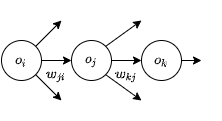
\includegraphics[scale = 0.6]{Images/flow_g.png}
    \caption{Network graph computation: $o_i$, $o_j$, $o_k$ are respectively the output of the  $i$-th input unit, $j$-th hidden unit and  $k$-th output unit. $w_{ji}$ is the weight associated with node $j$ connected to input $i$ (same for $w_{kj}$)}.
    \label{fig:computation_graph_backProp}
\end{figure}
\noindent The signal flow through the network in a forward direction as shown in Fig. \ref{fig:computation_graph_backProp} and a generic unit $t$ will compute the output $o_t$ with its activation function $f_t$ after computing the $net_t$:
\begin{equation}
\label{eq:generic_unit_eq}
    \left\{
        \begin{array}{ll}
            net_t = \sum_{q} w_{tq}o_q\\
            o_t = f_t(net_t)
        \end{array}
    \right.
\end{equation}
With Eq. \ref{eq:nn_function}, \ref{eq:error_function} and \ref{eq:generic_unit_eq} we can write the gradient respect a generic weights $d$ of unit $t$ assuming a pattern $p$:
$$\nabla_{p} w_{td} = - \frac{\partial E_{p}}{\partial w_{td}} = - \frac{\partial E_{p}}{\partial net_t} \cdot \frac{\partial net_t}{\partial w_{td}} = \delta_{t} \cdot o_d$$
Where, $\delta_t$ is the delta of unit $t$ and $o_d$ is the  input from a generic unit $d$ to the unit $t$, since
\[
 \frac{\partial net_t}{\partial w_{td}} = \frac{\partial \sum_{q} w_{tq}o_q}{\partial w_{td}} = o_d
\]

\noindent Now let's see the development of $\delta_t$:

$$\delta_t = - \frac{\partial E_p}{\partial net_t} = - \frac{\partial E_p}{\partial o_t} \cdot \frac{\partial o_t}{\partial net_t} = - \frac{\partial E_p}{\partial o_t} \cdot f'_t(net_t)$$
Where $- \frac{\partial E_p}{\partial o_t}$ changes according to the type of unit:

\begin{itemize}
    \item \textbf{Out unit K}
    $$- \frac{\partial E_p}{\partial o_k} = - \frac{\partial \frac{1}{2} \sum_{r}(d_{r}-o_{r})^2}{\partial o_{k}} = (d_{k}-o_{k})$$ 
    
    \item \textbf{Hidden unit J}
    $$- \frac{\partial E_p}{\partial o_j} = \sum_{k} - \frac{\partial E_p}{\partial net_k}\cdot \frac{\partial net_k}{\partial o_j} = \sum_{k} \delta_k \cdot w_{kj}$$ 
    \[
    \text{Since}\left\{
        \begin{array}{ll}
            - \frac{\partial E_p}{\partial net_k} = \delta_k \quad \text{(already computed)}\\
            \frac{\partial net_k}{\partial o_j} = \frac{\partial \sum_{R}^{}w_{kR}o_R}{\partial o_j} = w_{kj}
        \end{array}
    \right. 
\]

It expresses the variation of $E$ with respect to all the output unit $o_k$. Each $o_k$ (and $net_k$) depends on $o_j$, hence we introduce a sum over $k$.
\end{itemize}

\noindent \textbf{Summary}: We derived the gradient for a generic unit $t$ with input from $o_d$
$$ \nabla_p w_{ti} = \delta_t o_d$$
\begin{itemize}
    \item IF $t = k$ (output unit)
        \begin{equation}
            \label{eq:g_output_unit}
            \delta_k = (d_k - o_k)f_k^{'}(net_k)
        \end{equation}
    \item IF $t = j$ (hidden unit)
        \begin{equation}
            \label{eq:g_hidden_unit}
            \delta_j = \left( \sum_{k}^{}\delta_k w_{kj} \right) f_j^{'}(net_j)
        \end{equation}

\end{itemize}

\noindent This process can be generalised to $m$ hidden layers. Deltas come not only from the output layer but also from any up-layer to the considered layer in the computational graph. In other words, deltas flow from any units to which the considered unit is connected to and this is the reason why this process is called \textbf{Backpropagation}.

\subsection{Loss function: enforce Lipschitz continuity on the gradient}
\label{sec:l_lips_g}
From the analysis made it is clear that the neural network lives in a non-convex domain and we have to solve a non-linear unconstrained optimization problem. Both algorithms, that will be discussed in the next sections, require that the objective function gradient is global Lipschitz continuous for the global convergence analysis. Looking at the result found in the backpropagation it is immediately clear that it is not possible to take this property into account. 
To better understand why this is not true, let's understand which functions are Lipschitz continuous if we consider the product and the linear combination of two Lipschitz continuous functions.\\

Lipschitz continuity is designed to measure change of function values versus change in the independent variable for a general function\footnote{In practical implementations, with the typical floating point numbers, instead: $f \;:\; I \rightarrow Q$ where I is a set of rational numbers.} $f \;:\; I \subseteq \mathbb{R}^n \rightarrow \mathbb{R}^m$:
\begin{theorem}
\label{th:l_sum}
Suppose that $f_1,..., f_n$ are Lipschitz continuous on $I$ with Lipschitz constants  $L_1 , ... , L_n$ respectively. Then the linear combination $c_1f_1 +...+c_nf_n$ is Lipschitz continuous on $I$ with Lipschitz constant $c_1L_1 +...+ c_nL_n$.
\end{theorem}
\noindent If we consider the product of two Lipschitz continuous functions on a bounded set I:
\begin{theorem}
\label{th:l_prodoct}
If $f_1(x)$ and $f_2(x)$ are Lipschitz continuous on a bounded set $I$ then $f_1(x)f_2(x)$ is Lipschitz continuous on I.
\end{theorem}
\noindent By analyzing the individual components of the gradient, we can see that it does not always respect the Th. \ref{th:l_sum} and \ref{th:l_prodoct}. This can be seen immediately by looking at Eq. \ref{eq:g_hidden_unit}, where the partial derivative is a composition of products of bounded Lipschitz continuous functions and the weights that are not restricted within a bounded set. In fact, in a iterative algortithm the gradient will be computed $k$ times until a stop condition is reached, the gradient Lipschitz continuity can be considered true only on the first iteration since the the weights are generated by a bounded and closed set, as seen in \ref{sec:w_init}, but not in any further iterations.\\

\noindent To overcome this problem we can add a regularization term to the Error function and use this new objective function that, from now on, we will call Loss function:
\begin{equation}
    \label{eq:loss_f}
    L(\mathbf{w}) = E(\mathbf{w}) + \lambda\norm{\mathbf{w}}^2
\end{equation}

where $\norm{\cdot}$ denotes the Euclidean norm that allows the $L(\mathbf{w})$ to be still bounded below in $\mathbf{R}^n$  by zero and differentiable. Now, as will be shown in the further sections, due to the fact that the conjugate gradient and limited-memory quasi-Newton methods generate a monotonous decreasing sequence of values of the objective function, we can derive that:

$$L(\mathbf{w}_i) \leq L(\mathbf{w}_0)\; , \; \forall i \in (1,2,3, ...k)$$
$$E(\mathbf{w}_i) + \lambda \norm{\mathbf{w}_i}^2 \leq L(\mathbf{w}_0)$$
Since, $E(\mathbf{w})$ is bounded below to zero,  $E(\mathbf{w}_i)$ is a constant and at least it will be zero, we can write that:
$$\lambda \norm{\mathbf{w}_i}^2 \leq L(\mathbf{w}_0)$$
$$\norm{\mathbf{w}_i}^2 \leq \frac{L(\mathbf{w}_0)}{\lambda} $$
$$\norm{\mathbf{w}_i} \leq \sqrt{\frac{L(\mathbf{w}_0)}{\lambda}} $$

we have thus proved that, in this case, the weights are bounded and the gradient is Lipschitz continuous.\\

It is interesting to note that the regularization term is quite often used in the machine learning world and it allows to control the complexity of the model. Moreover, if the $\lambda$ constant is very low the weights will be subject to a very low or no regularization effect and they will be able to change arbitrarily (e.g. where a flexible model is needed it for a function approximation task). In this case, the error term will be the main part to be minimized to decrease the overall value of the loss, while still maintaining Lipschitz's continuous property on the gradient. Otherwise, with high $\lambda$ value the regularization term will be more important to minimise and it will lead to low weight and very rigid models.




\section{Nonlinear Conjugate Gradient Method}
\label{sec:NCG}
To improve the performances of a Neural Network, instead of using the simple steepest-descent algorithm, an interesting second-order optimizer can be used: the \emph{Conjugate Gradient} method. It was proposed by Hestenes and Stiefel \cite{Hestenes1952} in 1952 and extended to nonlinear functions by Fletcher and Reeves \cite{Fletcher1964} in 1964. This optimizer is faster than the steepest-descent and ensures low-memory requirements. The methods generate a sequence of weights $\{ \mathbf{w}_k \}$, for every iteration of training $k$, using the iterative formula
\begin{equation}
    \mathbf{w}_{k+1}=\mathbf{w}_k + \alpha_k \, \mathbf{d}_k, \,\,\, k=0,1,...,\label{eq:9}
\end{equation}
where $\alpha_k > 0$ is the step-length and $\mathbf{d}_k$ is a descent search direction. Hence the new weight update rule, as we can see from Algo. \ref{alg:conjugate}, will be
\begin{equation}
    \Delta \mathbf{w}_k = \alpha_k \mathbf{d}_k.
\end{equation}
\begin{algorithm}[H]
\label{alg:conjugate}
\SetAlgoLined
 \textbf{init}: starting point $\mathbf{w}_0$, $max\_iter$, $\varepsilon = 10^{-4}$, $k = 0$\;
 \While{k < max\_iter}{
  Evaluate the Loss function $L_k$ and its gradient $g_k$\;
  \If{$\norm{g_k} > \varepsilon$}{\textbf{return} Loss $L_k$}
  Compute $\beta_k$ with one of the methods PR, FR, HS\;
  Compute the descent direction $\mathbf{d}_k$ by \emph{conjugate direction}\;
  Compute the step-legnth $\alpha_k$ with a Line Search satisfying the Strong Wolfe conditions\;
  Update the weights $\mathbf{w}_{k+1} \leftarrow \mathbf{w}_k + \alpha_k \,\mathbf{d}_k$\;
  Set $k \leftarrow k + 1$\;
 }
 \caption{Nonlinear Conjugate Gradient}
\end{algorithm}
\vspace{+6pt}
\noindent By looking to the Algo. \ref{alg:conjugate} we can observe three main computation: $\beta_k$, descent direction $\mathbf{d}_k$ and the step-length $\alpha_k$. Let's see them in details.
\subsection{Search Direction}\label{search_direction}
The search direction, also called the \emph{conjugate direction}, at the k-th iteration is defined by
\begin{equation}\label{direction}
    \mathbf{d_k} = 
    \begin{cases}
        -\mathbf{g}_k, & \text{if } k=0 \\
        -\mathbf{g}_k + \beta_k \,  \mathbf{d}_{k-1}, & \text{if } k>0, 
    \end{cases} 
\end{equation}
where $\beta_k$ is a scalar that quantifies how much of the previous direction should be added to the new one, and $\mathbf{g}_k =\nabla L(\textbf{w}_k)$. Each new direction it's a linear combination of the steepest descent and the previous direction, hence the algorithm can compute a new vector $\mathbf{d}_k$ by only using the previous vector $\mathbf{d}_{k-1}$, and this is why it requires a little storage and computation. When dealing with quadratic functions, the method ensures that each direction is a descent direction. However, this not holds anymore for general nonlinear functions. In this case, to ensure that $\mathbf{d}_k$ will be a descent direction, $\alpha_k$ must satisfy certain conditions. Nevertheless, this may not be enough, and it is necessary to restart the process, how explained better in \ref{beta}.\\
%\cgv{\textbf{Pag.35}: it is not difficult to prove that there exist step lengths that satisfy Wolfe conditions for every function that is smooth and bounded below}

\subsection{Beta}\label{sec:beta}
There are different formulas for the computation of $\beta$. Each of them leads to different conjugate gradient methods with its computational efficiency and properties. The best-known formulas are called the Fletcher-Reeves (FR), Polak-Ribière (PR), and Hestenes-Stiefel (HS), and are given by 
\begin{equation}
  \beta_k^{FR} = \frac{\mathbf{g}_k^\mathsf{T} \, \mathbf{g}_k}{\mathbf{g}_{k-1}^\mathsf{T} \, \mathbf{g}_{k-1}},  
\end{equation}
\begin{equation}
  \beta_k^{PR} = \frac{\mathbf{g}_k^\mathsf{T} \, (\mathbf{g}_k - \mathbf{g}_{k-1})}{\|\mathbf{g}_{k-1}\|^2},  
\end{equation}
\begin{equation}
  \beta_k^{HS} = \frac{\mathbf{g}_k^\mathsf{T} \, (\mathbf{g}_k - \mathbf{g}_{k-1})}{(\mathbf{g}_k - \mathbf{g}_{k-1})^\mathsf{T} \, \mathbf{d}_{k-1}}.  
\end{equation}
As mentioned in \ref{search_direction}, with general nonlinear functions, $\mathbf{d}_k$ may fail to be a descent direction because of the second term in $\mathbf{d}_k = -\mathbf{g}_k + \beta_k\, \mathbf{d}_{k-1}$. For FR method is sufficient that $\alpha_k$ satisfies strong Wolfe conditions with $0 < c_1 < c_2 < \frac{1}{2}$ (we imposed $c_2 < \frac{1}{2}$ here, in place of the looser condition $c_2 < 1$ that was used in \ref{alpha}) to guarantee this property. However, this not hold for PR and HF methods. To overcome this problem, these methods, as suggested by Powell \cite{powell}, must be modified in
\begin{equation}\label{beta_modified}
  \beta = max\{\beta, \, 0\}.  
\end{equation}
This modification introduces a sort of restart of the algorithm, in case the $\beta$ found is negative. Indeed the algorithm puts aside the last search direction and restarts with the steepest descent.

\begin{comment}
One thing in common to these formulas, they must guarantee the global convergence of the method. Al-Baali \cite{baali} proved that the FR method with inexact line searches is globally convergent on general functions. Moreover, he showed that using strong Wolfe conditions always generates descent directions.  Instead, for the PR and HS method, the strong Wolfe conditions by themselves do not guarantee that $\textbf{d}_k$ is always a descent direction. So, when the function to be minimized is convex and quadratic, there are no problems and the Conjugate Gradient algorithm ensures the convergence in \emph{n} steps, however, when dealing with nonquadratic functions, like in this case, the direction computed could be not a descent direction. To overcome this issue, all the methods must be modified in
\begin{equation}\label{beta_modified}
  \beta = max\{\beta, \, 0\},  
\end{equation}
to ensure the global convergence. This modification introduces a sort of \emph{restart} of the algorithm, in case the $\beta$ found is negative. Indeed the algorithm puts aside the last search direction and restarts with the steepest descent.
\end{comment}

\subsection{Step-length}\label{alpha}
After the computation of the new direction $\mathbf{d}_k$, the step-length $\alpha_k > 0$ has to be found. The step-length is a simple scalar that, in the linear version of the method, was computed with a formula. However, in the nonlinear variant of the Conjugate Gradient, a line search has to be performed to find the right step size, which minimizes the Loss ($L$) function along $\mathbf{d}_k$., so
\begin{equation}\label{linesearch}
    \alpha_k = \min\limits_{\alpha} \,\, L(\mathbf{w}_k + \alpha \mathbf{d}_k).
\end{equation}
We could perform a \emph{exact line search} and find tThe best choice for $\alpha$ aswould be the global minimizer of Eq.(\ref{linesearch}), but this would take too much time. Even searching for a local minimizer would bee too expensive. Hence, the smarter way is to perform an \emph{inexact line search}, that tries out a sequence of candidate values for $\alpha$ and accepts the first one satisfying some conditions. In this way, we can obtain a relevant reduction of the Loss at a minimal cost.\\
This line search is done in two stages:
\begin{itemize}
    \item a \emph{bracketing phase}, that finds an interval containing step lengths that minimize the Loss;
    \item an \emph{interpolation phase} that, given the interval, finds an acceptable step length.
\end{itemize}
For our implementation, we decided for a line search that satisfies the \emph{Armijo-Wolfe} conditions. Those conditions are:
\begin{itemize}
    \item the \emph{sufficient decrease} condition (\emph{Armijo} condition)
    \begin{equation}
        L(\mathbf{w}_k + \alpha \, \mathbf{d}_k) \, \leq \, L(\mathbf{w}_k)\, + \, c_1 \, \alpha \, \mathbf{g}_k^\mathsf{T} \, \mathbf{d}_k,
    \end{equation}
    where $c_1 \in (0,1)$ is a constant, and  $\mathbf{g}_k^\mathsf{T}\mathbf{d}_k$ is the directional derivative. This condition, ensuring that the step-length $\alpha$ is not too large, forces a sufficient decrease in the function. However, alone it does not guarantee convergence, because it is satisfied for all sufficiently small values of $\alpha >0$. The constant $c_1$ has to be quite small, so it was set to $10^{-4}$. 
    \item the \emph{Strong Wolfe} condition
    \begin{equation}
        |\mathbf{g}(\mathbf{w}_k + \alpha \, \mathbf{d}_k)^\mathsf{T} \mathbf{d}_k|\, \leq  \, - c_2 \, \mathbf{g}_k^\mathsf{T} \, \mathbf{d}_k,
    \end{equation}
    where $c_2 \in (c_1,1)$ is a constant. This condition ensures that the slope of the function after moved by a step $\alpha$ (that is not too small because of this condition) along the direction $\mathbf{d}$ is greater than $c_2$ times the initial slope. In this case, the constant $c_2$ is equal to 0.1.  Moreover, the strong condition doesn't allow the derivative $\mathbf{g}(\mathbf{w}_k + \alpha \, \mathbf{d}_k)^\mathsf{T} \mathbf{d}_k$ to be too positive and ensures that $\alpha$ is close to a minimizer of the function.
\end{itemize}
Our algorithm implementation, which satisfies Strong Wolfe conditions, follows the one described in \cite{Nocedal} and is composed by two functions: \verb|line_search| and \verb|zoom|. They are both illustrated in Algo. \ref{algo:line_search} and \ref{algo:zoom} where it is assumed that: $\phi(\alpha) = L(\mathbf{w}_k + \alpha \mathbf{d}_k)$ and $\mathbf{d} = \mathbf{d}_k$. 

\begin{algorithm}[H]
\label{algo:line_search}
\SetAlgoLined
 \textbf{init}: $\alpha_0 \leftarrow 0$, choose $\alpha_{max} > 0$ and $\alpha_1 \in (0, \, \alpha_{max})$\;
 $i \leftarrow 1$\;
 \While{i < max\_iter}{
  Evaluate $\phi(\alpha_i)$\;
  \If{$[\phi(\alpha_i) > \phi(0) \, + \, c_1 \, \alpha_i \, \nabla \phi(0)^\mathsf{T}d] \,\, or \,\, [\phi(\alpha_i) \leq \phi(\alpha_{i-1}) \,\, and \,\, i > 1]$}{
  $\alpha_* \leftarrow \mathbf{zoom}(\alpha_{i-1}, \, \alpha_i)$\;
  \textbf{return} $\alpha_*$\;
  }
  Evaluate $\nabla \phi(\alpha_i)^\mathsf{T}d$\;
  \If{$|\nabla \phi(\alpha_i)^\mathsf{T}d| \leq -c_2 \, \nabla \phi(0)^\mathsf{T}d$}{
  $\alpha_* \leftarrow \alpha_i$\;
  \textbf{return} $\alpha_*$\;
  }
  \If{$\nabla \phi(\alpha_i)^\mathsf{T}d \geq 0$}{
  $\alpha_* \leftarrow \mathbf{zoom}(\alpha_i, \, \alpha_{i-1})$\;
  \textbf{return} $\alpha_*$\;
  }
  Choose $\alpha_{i+1} \in (\alpha_i, \, \alpha_{max})$\;
  $i \leftarrow i + 1$\;
 }
 \caption{Line Search}
\end{algorithm}

\begin{algorithm}[H]
\label{algo:zoom}
\SetAlgoLined
 \While{i < max\_iter}{
  $\alpha_j \leftarrow quadratic\_cubic\_interpolation(\alpha_{lo}, \, \alpha_{hi})$\;
  Evaluate $\phi(\alpha_j)$\;
  \eIf{$[\phi(\alpha_j) > \phi(0)\, +\, c_1 \, \alpha_j \, \nabla \phi(0)^\mathsf{T} \, d_0]\,\, or \,\,[\phi(\alpha_j) \leq \phi(\alpha_{lo})]$}{
  $\alpha_* \leftarrow \alpha_j$\;
  \textbf{return} $\alpha_*$\;
  }{
  Evaluate $\nabla \phi(\alpha_j)^\mathsf{T}d$\;
  \If{$|\nabla \phi(\alpha_j)^\mathsf{T} d|\leq - c_2 \, \nabla \, \phi(0)^\mathsf{T} \, d$}{
  $\alpha_* \leftarrow \alpha_j$\;
  \textbf{return} $\alpha_*$\;}
  \If{$\nabla \phi(\alpha_j)^\mathsf{T}d\,(\alpha_{hi} - \alpha_{lo}) \geq 0$}{
  $\alpha_{hi} \leftarrow \alpha_{lo}$\;}
  }
  Set $\alpha_{lo} \leftarrow \alpha_j$\;
  $i \leftarrow i + 1$\;
 }
 \caption{zoom}
\end{algorithm}

\subsection{Convergence Analysis}\label{global_convergence}
In Sec.~\ref{sec:beta} several beta formulas have been presented and each of them requires a different theoretical analysis. As discussed in \cite{nocedal_global_convergence} the Fletcher-Reeves \cite{Fletcher1964} method can be as efficient as the Polak-Ribire and Hestenes Stiefel methods, but it is often much slower and erratic. Moreover, as shown by Powell \cite{Powell1977}, the Fletcher-Reeves, under some circumstances, can produce very small displacements and it needs some restart along the gradient direction in order to recover. Despite these drawbacks, Zoutendijk
\cite{zoutendijk1970northholland} has shown that the method cannot fail. He proved that the Fletcher-Reeves
method with exact line searches is globally convergent on general functions. Al-Baali \cite{baali} extended this result to inexact line searches. For the purposes of this section, we make the following assumptions on the objective function.
\begin{assumption}
\label{as:1}
The level set $\mathcal{L} = \{ \mathbf{w}\, | \, L(\mathbf{w}) \leq L(\mathbf{w}_0)\}$ is bounded, namely, there exists a constant $B > 0$ such that:
$$ \norm{\mathbf{w}} \leq B, \; \forall i \in \mathcal{L}$$ 
\end{assumption}
\begin{assumption}
\label{as:2}
    In some neighborhood $\mathcal{N}$ of $\mathcal{L}$, the objective function L is continuously differentiable, and its gradient is Lipschitz continuous, there exists a constant $C > 0$ such that 
    $$
      \|\mathbf{g}(\textbf{w}) - \mathbf{g}(\tilde{\textbf{w}})\| \, \leq \,  C \| \mathbf{w} - \tilde{\mathbf{w}}\|,\; \forall \mathbf{w}, \tilde{\mathbf{w}} \in \mathcal{N}
    $$
    It follows directly from 1 and 2 that there exists a positive constant $\gamma>0$ such that:
    $$\norm{\mathbf{g}(\textbf{w})} \, \leq\, \gamma, \;\; \forall \mathbf{w} \in \mathcal{L} $$
\end{assumption}
\noindent Since the function L defined in Eq. \ref{eq:loss_f} is bounded below in $\mathbf{R}^n$  by zero and it has been proved, in Sec. \ref{sec:l_lips_g}, that due to the monotonic property of the algorithm $\norm{\mathbf{w}_i} \leq \sqrt{\frac{L(\mathbf{w}_0)}{\lambda}} $ for all $i$ such that $L(\mathbf{w}_i) \leq L(\mathbf{w}_0)$. Moreover, the direct consequence, given the composition of the gradient, is that the gradient of the loss function is Lipschitz continuous. So, Assumption \ref{as:1} and \ref{as:2} always hold.

\subsubsection{Global convergence of the Fletcher-Reeves method}
As regards the FR method, we saw in \ref{search_direction} that $\mathbf{d}_k$ is a descent direction if $\alpha_k$ satisfies strong Wolfe with $0 < c_1 < c_2 < \frac{1}{2}$. So the global convergence of the algorithm is guaranteed by the Al-Baali theorem \ref{th:FR_convergence}.
\begin{theorem}(Al-Baali \cite{baali})\\
\label{th:FR_convergence}
If Assumptions \ref{as:1} and \ref{as:2} hold, and that Algorithm \ref{alg:conjugate} is implemented with a line search that satisfies the strong Wolfe conditions, with $0 < c_1 < c_2 < \frac{1}{2}$. Then
\begin{equation}
      \lim_{k\to\infty} \mathrm{inf} \, \|\mathbf{g}_k\| = 0.
\end{equation}
\end{theorem}

\subsubsection{Global convergence of Polak-Ribière and Hestenes-Stiefel methods }
Instead, for PR and HS methods, if we use $\beta$ modified as in Eq. \ref{beta_modified} to guarantee a descent direction, and a Line Search as described in \ref{alpha} to find $\alpha_k$, then, an important result from the Gilbert and Nocedal theorem proving global convergence in \cite{nocedal_global_convergence} is the following corollary.
\begin{corollary}
Suppose that Assumptions \ref{as:1} and \ref{as:2} hold. Consider the method with $\beta = max\{\beta, \, 0\}$, and with a line search satisfyng the strong Wolfe conditions. Then
\begin{equation}
      \lim_{k\to\infty} \mathrm{inf} \, \|\mathbf{g}_k\| = 0.
\end{equation}
\end{corollary}
\noindent So the global convergence is also guaranteed for those beta methods.
\cac{questo ci porta ad avere l'algo che termina in n passi(?)}
\begin{comment}
So, if we use $\beta$ modified as in Eq. \ref{beta_modified}, and a Line Search as described in \ref{alpha} to find $\alpha_k$, then, how explained by Gilbert and Nocedal in \cite{nocedal_global_convergence}, the global convergence of the algorithm holds. Hence we have
\begin{equation}
      \lim_{k\to\infty} \mathrm{inf} \, \|\mathbf{g}_k\| = 0.
\end{equation}
\end{comment}

\section{Limited-Memory BFGS Method}\label{sec:QNM}
The conjugate gradient has led us to nice properties and faster convergence than the classic gradient descent method. Another class of optimization algorithms is the \emph{quasi-Netwon methods}, that are characterized by further interesting convergence properties such as \emph{superlinear convergence}.

The first quasi-Newton method was developed by W. C. Davidon in 1959 \cite{davidon}, and, like steepest descent, only the gradient must be provided at each iteration \cite{Nocedal} and allows to avoid the direct computation of the hessian, not feasible to compute in some problem and required in the Newton method. By measuring the changes in gradients, it constructs a model of the objective function that is good enough to produce superlinear convergence. In 1963 Fletcher and Powell \cite{10.1093/comjnl/6.2.163} have demonstrated theoretically and with numerical examples that it was considerably superior to other previously methods available at that time - It transformed the nonlinear optimization. In fact, the improvement over steepest descent was dramatic and this is the reason why, over the years, several variants of this method were proposed to achieve even better results in the nonlinear optimization. The most popular quasi-Newton algorithm is the \emph{Broyden–Fletcher–Goldfarb–Shanno (BFGS)} method, where each step has the form
\begin{equation}
    \mathbf{w}_{k+1}=\mathbf{w}_k + \alpha_k \, \mathbf{d}_k,
    \label{eq:bfgs_update}
\end{equation}
where $\alpha_k$ is the step lenght chosen to satisfy strong Wolfe conditions (see Section \ref{alpha}), and $\mathbf{d}_k$ is the search direction defined by
\begin{equation}
    \mathbf{d}_k = - \mathbf{H}_k \, \mathbf{g}_k,
    \label{eq:d_bfgs}
\end{equation}
where $\mathbf{H}_k$ is the inverse of the approximation $\mathbf{B}_k$ of the Hessian (the Hessian is $\nabla^2 L_k$). Given an initial fixed $\mathbf{H}_0$, chosen with some heuristic \cite{Nocedal}, $\mathbf{H}_k$ it is updated at every iteration by formula
\begin{equation}
    \mathbf{H}_{k+1}=\mathbf{V}_k^\mathsf{T} \, \mathbf{H}_k \, \mathbf{V}_k + \rho_k \, \mathbf{s}_k \, \mathbf{s}_k^\mathsf{T},
    \label{eq:bfgs_H_update}
\end{equation}
where 
\begin{equation}
    \rho_k = \frac{1}{\mathbf{y}_k^\mathsf{T} \, \mathbf{s}_k}, \,\,\,\,\,\,\,\, \mathbf{V}_k = \mathbf{I} \, - \, \rho_k \, \mathbf{y}_k \, \mathbf{s}_k^\mathsf{T},
    \label{}
\end{equation}
and
\begin{equation}
    \mathbf{s}_k = \mathbf{w}_{k+1} - \mathbf{w}_k, \,\,\,\,\,\,\,\, \mathbf{y}_k = \mathbf{g}_{k+1} - \mathbf{g}_k.
    \label{}
\end{equation}
The updated approximation $\mathbf{H}_{k+1}$ must be symmetric and positive definite, and must satisfy the \emph{secant equation}
\begin{equation}
    \mathbf{H}_{k+1} \mathbf{y}_k = \mathbf{s}_k.
    \label{secant_equation}
\end{equation}
This is possible only if $\mathbf{s}_k$ and $\mathbf{y}_k$ satisfy the \emph{curvature condition}
\begin{equation}
    \mathbf{s}_k^\mathsf{T}\mathbf{y}_k > 0.
    \label{curvature_condition}
\end{equation}
For nonconvex functions, like in our case, the inequality (\ref{curvature_condition}) is guaranteed to hold if we impose the strong Wolfe conditions on the line search that chooses $\alpha_k$.\\

However, even if BFGS solves the problem of the Hessian calculation by replacing it with an approximation, this method can be only used in an unconstrained optimization problem where the number of variables allows us to keep computational cost and storage feasible. The Hessian approximations generated by the quasi-Newton, as BFGS, are usually dense, even when the true Hessian is sparse, and with $n$ variables they require $O(n^2)$ in storage complexity. Many applications raise unconstrained optimization problems with thousands or millions of variables, as in a neural network model, and those approaches become unfeasible to use.\\

%%\textbf{L-BFGS}\\
Since our objective function lies in the case of large scale optimization problem, here will take in analysis the study of a limited-memory quasi-Newton method, useful when Hessian matrices cannot be computed at a reasonable cost or are not sparse (respectively problems occurred in Newton and quasi-Netwon methods), known as the \emph{limited-memory BFGS} (L-BFGS). This method stores a \emph{modified} version of $\mathbf{H}_k$ \emph{implicitly} in a compact way by using just a finite number ($m$) of vector pairs $\{ \mathbf{s}_i, \, \mathbf{y}_i\}$. The $m$ value can be controlled by the user to manage the trade-off between the storage complexity and better approximation of the Hessian.\\

The L-BFGS has the same update rule of the BFGS for the next iterate (Eq. \ref{eq:bfgs_update}), but it differs on the $\mathbf{H}_k$ computation in Eq. \ref{eq:d_bfgs} and in the choice of the initial matrix $\mathbf{H}_0$ (that is allowed to vary from iteration to iteration). The algorithm will now be shown in Algo. \ref{alg:bfgs} and in the next sections, we will focus on deriving the search direction and the step length for the limited version.

\begin{algorithm}[H]
\label{alg:bfgs}
\SetAlgoLined
 \textbf{init}: starting point $\mathbf{w}_0$, $max\_iter$, $m  > 0$\;
 $k \leftarrow 0$\;
 \While{k < max\_iter}{
  Choose the initial matrix $\mathbf{H}_k^0$\;
  Compute the search direction $\textbf{d}_k \leftarrow -\mathbf{H}_k \, \mathbf{g}_k$ with the L-BFGS formula\;
  Compute the step length $\alpha_k$ with a Line Search satisfying the Strong Wolfe conditions\;
  Update the weights $\mathbf{w}_{k+1} \leftarrow \mathbf{w}_k + \alpha_k \mathbf{d}_k$\;
  \If{$k > m$}{
  Discard the oldest vector pair $\{ \mathbf{s}_{k-m}, \, \mathbf{y}_{k-m}\}$ from storage\;}
  Compute and save $\mathbf{s}_k \leftarrow \mathbf{w}_{k+1} - \mathbf{w}_k$, $\mathbf{y}_k = \mathbf{g}_{k+1} - \mathbf{g}_k$\;
  Set $k \leftarrow k + 1$\;
 }
 \caption{L-BFGS}
\end{algorithm}


\subsection{Search Direction}
\label{sec:search_dir_qn}
The product $\mathbf{H}_k\mathbf{g}_k$ in Eq.\ref{eq:d_bfgs} can be obtained by a recursive formula involving a sequence of inner products and vector summations of the gradient $\mathbf{g}_k$, an initial inverse Hessian approximation $\mathbf{H}^0_k$ and the set of vector pairs $\{ \mathbf{s}_i, \, \mathbf{y}_i\}$ that includes curvature information from the $m$ most recent iterations that reduce to memory complexity. Indeed, after each iteration, the oldest vector pair $\{ \mathbf{s}_i, \, \mathbf{y}_i\}$ is replaced by the new one obtained at the current iteration $\{ \mathbf{s}_k, \, \mathbf{y}_k\}$. By combining everything, we can repeat the Eq. \ref{eq:bfgs_H_update} and derive the following L-BFGS approximation $\mathbf{H}_k$:
\begin{equation}
\begin{split}
     \mathbf{H}_k = \,&(\mathbf{V}_{k-1}^\mathsf{T}\, .\,.\,.\, \mathbf{V}_{k-m}^\mathsf{T})\,\mathbf{H}_k^0\,(\mathbf{V}_{k-m}\,.\,.\,.\, \mathbf{V}_{k-1})\\
    & + \rho_{k-m}\,(\mathbf{V}_{k-1}^\mathsf{T}\,.\,.\,.\,\mathbf{V}_{k-m+1}^\mathsf{T})\, \mathbf{s}_{k-m}\mathbf{s}_{k-m}^\mathsf{T} \, (\mathbf{V}_{k-m+1}^\mathsf{T}\,.\,.\,.\,\mathbf{V}_{k-1}^\mathsf{T})\\
    & + \rho_{k-m+1}\,(\mathbf{V}_{k-1}^\mathsf{T}\,.\,.\,.\,\mathbf{V}_{k-m+2}^\mathsf{T})\,\mathbf{s}_{k-m}\mathbf{s}_{k-m+1}^\mathsf{T} \,(\mathbf{V}_{k-m+2}^\mathsf{T}\,.\,.\,.\,\mathbf{V}_{k-1}^\mathsf{T})\\
    & + .\,.\,.\\
    & + \rho_{k-1}\mathbf{s}_{k-1}\mathbf{s}_{k-1}^\mathsf{T}.
\end{split}
\label{eq:LBFGS_H_update}
\end{equation}
Eq. \ref{eq:LBFGS_H_update} leads to Algo. \ref{alg:bfgs_loop} that allows recursively computing product $\mathbf{H}_k \, \mathbf{g}_k$.

\begin{algorithm}[H]
\label{alg:bfgs_loop}
\SetAlgoLined
 $\mathbf{q} \leftarrow \mathbf{g}_k$ \;
 \For{$i = k-1, \,\, k-2, \,\, ... \,\, , \,\, k-m$}
    {$\alpha_i \leftarrow \rho_i \, \mathbf{s}_i^\mathsf{T} \, \mathbf{q}$\;
    $\mathbf{q} \leftarrow \mathbf{q} - \alpha_i \, \mathbf{y}_i$\;} 
 \EndFor
 $\mathbf{r} \leftarrow \mathbf{H}_k^0 \, \mathbf{q}$\;
 \For{$i = k-m, \,\, k-m+1, \,\, ... \,\, , \,\, k-1$}
    {$\beta \leftarrow \boldsymbol\rho_i \, \mathbf{y}_i^\mathsf{T} \mathbf{r} $\;
    $\mathbf{r} \leftarrow \mathbf{r} + \mathbf{s}_i(\alpha_i - \beta)$\;} 
 \EndFor
 \textbf{return} $\mathbf{H}_k \, \mathbf{g}_k = \mathbf{r}$
 \caption{L-BFGS two-loop recursion}
\end{algorithm}
Alg. \ref{alg:bfgs_loop} has a $O(mn)$ computational complexity, where $m$ is the number of vector pair stored in memory.\\

To ensure that $\mathbf{d}_k$ will be a \emph{descent direction}, $\mathbf{H}_{k+1}$ must be \emph{positive-definite}. \cgv{così è più chiaro?} As shown by Nocedal in \cite{Nocedal}, this holds whenever $\mathbf{H}_k$ (previous approximation) is positive definite, and the condition (\ref{curvature_condition}) is verified. Hence, if the initial approximation $\mathbf{H}^0_k$ is positive definite and the curvature condition is satisfied at every k step of the L-BFGS algorithm, $\mathbf{H}_{k}$ will be positive definite. As said before, the curvature condition is guaranteed because the line search satisfies the strong Wolfe conditions. Moreover, the initial Hessian was always the identity matrix ($\mathbf{I}$ is positive definite), and after one iteration was completed, we change the provisional value by setting
\begin{equation}\label{initial_matrix}
    \mathbf{H}_k^0 = \gamma_k \, \mathbf{I} = \frac{\mathbf{s}_{k-1}^\mathsf{T} \mathbf{y}_{k-1}}{\mathbf{y}_{k-1}^\mathsf{T}\mathbf{y}_{k-1}} \,\mathbf{I},
\end{equation}
which ensures that $\mathbf{H}_k^0$ is positive definite if (\ref{curvature_condition}) holds. The scaling factor $\gamma_k$ attempts to estimate the size of the true Hessian matrix along the most recent search direction (allowing $\mathbf{H}_k^0$ to vary between iterations). This choice helps to ensure that the search direction $\mathbf{d}_k$ is well scaled, and as a result the step length $\alpha_k = 1$ is accepted in most iterations. \cgv{non so, mi sembra di spiegare l'ovvio, ma se a lui non è chiaro non so che altro scrivere, in realtà mi viene da pensare che questa parte non l'abbia proprio letta, ho visto che tutti la spiegano così la positive definite (cioè non aggiungono altro). Mi sembra scritto di cacca}

\begin{comment}
As shown in \cite{Nocedal}, this holds when the initial approximation $\mathbf{H}_{0}$ is positive definite, and the \emph{curvature condition} $\mathbf{s}_k^\mathsf{T}\mathbf{y}_k > 0$ is verified. As said before, when dealing with non-convex functions, the curvature condition will be guaranteed if we impose that the line search satisfies the strong Wolfe conditions. In our case, the initial approximation $\mathbf{H}^0_k$ is positive-definite (is chosen has a multiple of the identity), and the curvature condition is satisfied at every iteration $k$, so $\mathbf{d}_k$ is a descent direction.
An efficient method for choosing the initial matrix $\mathbf{H}^0_k$ is

  \begin{equation}\label{initial_matrix}
      \mathbf{H}_k^0 = \gamma_k \, \mathbf{I} = \frac{\mathbf{s}_{k-1}^\mathsf{T} \mathbf{y}_{k-1}}{\mathbf{y}_{k-1}^\mathsf{T}\mathbf{y}_{k-1}} \,\mathbf{I}
  \end{equation}
\noindent where $\gamma_k$ is the scaling factor that attempts to estimate the size of the true Hessian matrix along the most recent search direction (allowing $\mathbf{H}_k^0$ to vary between iterations). This choice helps to ensure that the search direction $\mathbf{d}_k$ is well scaled, and as a result the step length $\alpha_k = 1$ is accepted in most iterations.
\end{comment}


\subsection{Step-length}\label{alpha_qn}
\cgv{Pensare di togliere questa sezione}\\
As noted above, a line search satisfying the \emph{strong Wolfe conditions}, with $0 \leq c_1 \leq c_2 \leq 1$, has to be performed to find the right step length $\alpha_k > 0$. The procedure, described in \ref{alpha}, is the same used for the conjugate gradient method. However, in this case, the constant $c_2$ is equal to 0.9 and, step $\alpha_0 = 1$ should always be used as the initial trial step length. Furthermore, the satisfaction of strong Wolfe conditions makes L-BFGS updating stable.

\subsection{Global convergence}\label{global_convergence_qn}
\cgv{Dobbiamo dire perché non abbiamo la convergenza globale.}\\
\cgv{Common theoretical results for L-BFGS merely show
that if the Hessian  approximations are sufficiently positive definite and bounded, then one can achieve a local linear rate of convergence}\\

\subsection{Superlinear convergence}\label{superlinear_convergence_qn}
\cgv{\textbf{FRANGIONI:} Intanto c'è da distinguere tra convergenza globale e velocità di convergenza superlineare. "Primum vivere", quindi la prima cosa da discutere è se si ha convergenza, indipendentemente dalla velocità; questo voi non lo discutete. Tra l'altro, l'assunzione che $B_k$ sia semidefinita positiva in generale è "gratis", ma anche questo non lo dite chiaramente.}\\
\cgv{\textbf{FRANGIONI:} Una volta chiarito se il metodo converge oppure no, va benissimo discutere la convergenza superlineare (ma in questo caso, perché non avete discusso la velocità di convergenza del NCG?). Che si può anche non riuscire a dimostrare, ma ... potrebbe non essere troppo difficile capire se l'Hessiano è bounded (su un insieme bounded), se uno quantomeno lo calcolasse. Insomma "Eq. 30 cannot be proved" sembra un po' strano: perché "cannot"? Ci avete provato? Se no, può anche andare bene, ma almeno ammettete che non avete avuto voglia di fare i conti anche se ci avreste potuto provare.}\\
In this section we present a convergence result for the L-BFGS method. As shown by Liu and Nocedal in \cite{Liu}, the L-BFGS method is globally convergent on uniformly convex problems,  but for general nonlinear objective functions, we will not be able to establish that. However, it is possible to prove the local \emph{superlinear convergence} of the method, under reasonable assumptions, even in the nonconvex case. For the purposes of this section, we make the following assumptions on the objective functon.
\begin{assumption}
\label{as:3}
The objective function is twice continuously differentiable. 
\end{assumption}
\begin{assumption}
\label{as:4}
The Hessian $\mathbf{B}_k$ need to be positive definite in order to have descent direction.
\end{assumption}

\noindent Sec. \ref{sec:error_f} shows that our objective function is twice differentiable and in Sec. \ref{sec:search_dir_qn} we've shown how the inverse Hessian approximation $\mathbf{H}_k$ can be computed in order to obtain a positive definite matrix at each iteration (the same is proved for the hessian $\mathbf{B}_k$ in \cite{Nocedal}). So assumption \ref{as:3} and \ref{as:4} holds.\\

An important result for our analysis comes from the convex case. The Theorem \ref{th:superlinearl_qn}, which ensures that a superlinear convergence rate can be obtained even if the sequence of quasi-Newton matrices $\mathbf{B}_k$ does not converge to $\nabla^2 L(\mathbf{w}^*)$. It sufficient that the $\mathbf{B}_k$ becomes increasingly accurate approximations to $\nabla^2 L(\mathbf{w}^*)$ \emph{along the search direction $\mathbf{d}_k$}.

\begin{theorem}
\label{th:superlinearl_qn}
Suppose $L$ is twice continuously differentiable. Consider the iteration $\mathbf{w}_{k+1}=\mathbf{w}_k + \alpha_k \mathbf{d}_k$, where $\mathbf{d}_k$ is a descent direction and $\alpha_k$ satisfies the strong Wolfe conditions with $c_1 \leq \frac{1}{2}$. If the sequence $\{ \mathbf{w}_k\}$ converges to a point $\mathbf{w^*}$ such that $\nabla L (\mathbf{w}^*) = 0$ and $\nabla^2 L(\mathbf{w}^*)$ is positive definite, and i the search direction satisfies
\begin{equation}
      \lim_{k\to\infty} \frac{\| \nabla L_k - \nabla^2 L_k \, \mathbf{d}_k\|}{\| \mathbf{d}_k\|} = 0,
\end{equation}
then
\begin{itemize}
    \item the step length $\alpha_k = 1$ is admissible for all $k>k_0$; and
    \item if $\alpha_k = 1$ for all $k>k_0$, $\{ \mathbf{w}_k\}$ converges to $\mathbf{w}^*$ superlinearly. 
\end{itemize}
\end{theorem}
Since $\mathbf{d}_k$ is a quasi-Newton search direction in the form of $\mathbf{d}_k = - \mathbf{B}_k^{-1} \, \mathbf{g}_k$, then (30) is equivalent to
\begin{equation}
      \lim_{k\to\infty} \frac{\| (\mathbf{B}_k - \nabla^2 L(\mathbf{w}^*)) \, \mathbf{d}_k\|}{\| \mathbf{d}_k\|} = 0.
\end{equation}
Condition (29) is \emph{both necessary and sufficient} for the superlinear convergence of quasi-Newton methods in the convex case. However, for the nonconvex analysis, this limit is not sufficient, and other assumptions are needed to guarantee the superlinear convergence.\\ 

Another useful result of the global convergence of L-BFGS, in the convex case, is displayed in \cite{Nocedal} and shows that the sequence $\| \mathbf{w}_k - \mathbf{w}^*\|$ converges to zero rapidly enough that
\begin{equation}\label{eq:seq_to_zero_rapidly}
    \sum_{k=1}^{\infty} \| \mathbf{w}_k - \mathbf{w}^*\| < \infty,
\end{equation}
where $\mathbf{w}^*$ is a minimizer of L and if it's hold can be proved that the rate of
convergence is actually superlinear.\\

\noindent Now, we can move to the superlinear convergence analysis valid for convex and non-convex cases. We need to make the following additional assumption.
\begin{assumption}
\label{as:5}
The Hessian matrix $\mathbf{G}$ is Lipschitz continuous at $\mathbf{w}^*$, that is,
\begin{equation}\label{eq:hessian_Lcontinuity}
    \| \mathbf{G}(\mathbf{w}) - \mathbf{G}(\mathbf{w}^*) \| \leq L\,\|\mathbf{w} - \mathbf{w}^*\|,
\end{equation}
for all $\mathbf{w}$ near $\mathbf{w}^*$, where L is a positive constant. 
\end{assumption}

Eq. \ref{eq:seq_to_zero_rapidly} and Assumption \ref{as:5} play an important role in superlinear convergence, as we now show. The proof of Assumption \ref{as:5} is provided in \cite{Nocedal} but Eq. \ref{eq:seq_to_zero_rapidly} cannot be proved in our non-convex analysis. So, for our purpose we assume, for now, that it holds and the local superlinear convergence of the L-BFGS algorithm is guaranteed by Theorem \ref{th:superlinearl_nonconvex}.
\begin{theorem}
\label{th:superlinearl_nonconvex}
Suppose that $L$ is twice continuously differentiable and that the iterates generated by BFGS algorithm converge to a minimizer $\mathbf{w^*}$ at which Assumption \ref{as:5} holds. Suppose also that (\ref{eq:seq_to_zero_rapidly}) holds. Then $\mathbf{w}_k$ converges to $\mathbf{w^*}$ at a superlinear rate.
\end{theorem}

The Theorem \ref{th:superlinearl_qn} and the limit (31) imply that the step length $\alpha_k = 1$ will satisfy the strong Wolfe conditions near the solution, and hence that the rate of convergence is superlinear. Anyway, Eq. \ref{eq:seq_to_zero_rapidly} doesn't hold in our specific case, we cannot demonstrate the superlinearity theoretically but we can practically observe it in the experiments section.  



\begin{comment}
\begin{assumption}
\label{as:3}
The objective function is twice continuously differentiable. 
\end{assumption}
\begin{assumption}
\label{as:4}
$\mathbf{H}_k$ need is positive definite.
\end{assumption}
\cgv{Spiegare perché le due assunzioni sono verificate.}\\

\cgv{Theorem 3.6 a pag.46}
\begin{theorem}
\label{th:superlinearl_qn}
Suppose $L$ is twice continuously differentiable. Consider the iteration $\mathbf{w}_{k+1}=\mathbf{w}_k + \alpha_k \mathbf{d}_k$, where $\mathbf{d}_k$ is a descent direction and $\alpha_k$ satisfies the strong Wolfe conditions with $c_1 \leq \frac{1}{2}$. If the sequence $\{ \mathbf{w}_k\}$ converges to a point $\mathbf{w^*}$ such that $\nabla L (\mathbf{w}^*) = 0$ and $\nabla^2 L(\mathbf{w}^*)$ is positive definite, and i the search direction satisfies
\begin{equation}
      \lim_{k\to\infty} \frac{\| \nabla L_k - \nabla^2 L_k \, \mathbf{d}_k\|}{\| \mathbf{d}_k\|} = 0,
\end{equation}
then
\begin{itemize}
    \item the step length $\alpha_k = 1$ is admissible for all $k>k_0$; and
    \item if $\alpha_k = 1$ for all $k>k_0$, $\{ \mathbf{w}_k\}$ converges to $\mathbf{w}^*$ superlinearly. 
\end{itemize}
\end{theorem}
\cgv{Allineare}\\
Since $\mathbf{d}_k$ is a quasi-Newton search direction in the form of $\mathbf{d}_k = - \mathbf{B}_k^{-1} \, \mathbf{g}_k$, then (27) is equivalent to
\begin{equation}
      \lim_{k\to\infty} \frac{\| (\mathbf{B}_k - \nabla^2 L(\mathbf{w}^*) \, \mathbf{d}_k) \mathbf{d}_k\|}{\| \mathbf{d}_k\|} = 0.
\end{equation}
Therefore, is sufficient that the $\mathbf{B}_k$ become increasingly accurate approximations to $\nabla^2 L(\mathbf{w}^*)$ along the search direction $\mathbf{d}_k$ to guarantee the superlinear convergence rate.

\cgv{Theorem 3.7 a pag.47}
\begin{theorem}
\label{th:superlinearl_qn}
Suppose $L$ is twice continuously differentiable. Consider the iteration $\mathbf{w}_{k+1}=\mathbf{w}_k + \mathbf{d}_k$ (that is, the step length $\alpha_k$ is uniformly 1) and that $\mathbf{d}_k$ is given by $\mathbf{d}_k = - \mathbf{B}_k^{-1} \, \mathbf{g}_k$. Let us assume also that $\{ \mathbf{w}_k\}$ converges to a point $\mathbf{w^*}$ such that $\nabla L (\mathbf{w}^*) = 0$ and $\nabla^2 L(\mathbf{w}^*)$ is positive definite. Then $\{ \mathbf{w}_k\}$ converges superlinearly if and only if (28) holds.
\end{theorem}

\cgv{Theorem 6.5 a pag.154-155-156}
\begin{theorem}
\label{th:superlinearl_convex}
Let $\mathbf{B}_0$ be any symmetric positive definite initial matrix, and let $\mathbf{w}_0$ be a starting point for which Assumption \ref{as:3} and Assumption \ref{as:4} are satisfied. Then the sequence $\mathbf{w}_k$ generated by Algorithm \ref{alg:bfgs} converges to the minimizer $\mathbf{w^*}$ of $L$.
\end{theorem}

Theorem \ref{th:superlinearl_convex} shows that the rate of convergence of the iterates is linear. In particular, the sequence $\| \mathbf{w}_k - \mathbf{w_0}\|$ converges to zero rapidly enough that 
\begin{equation}\label{eq:seq_to_zero_rapidly}
    \sum_{k=1}^{\infty} \| \mathbf{w}_k - \mathbf{w_0}\| < \infty.
\end{equation}

\cgv{Assumption 6.2 a pag.156}
\begin{assumption}
\label{as:5}
The Hessian matrix $G$ is Lipschitz continuous at $x^*$, that is,
\begin{equation}\label{eq:hessian_Lcontinuity}
    \| G(x) - G(x^*) \| \leq L\,\|x - x^*\|,
\end{equation}
for all x near x^*, where L is a positive constant.
\end{assumption}

\cgv{Theorem 6.6 a pag.158}
\begin{theorem}
\label{th:superlinearl_nonconvex}
Suppose that $L$ is twice continuously differentiable and that the iterates generated by BFGS algorithm converge to a minimizer $\mathbf{w^*}$ at which Assumption \ref{as:5} holds. Suppose also that (\ref{eq:seq_to_zero_rapidly}) holds. Then $\mathbf{w}_k$ converges to $\mathbf{w^*}$ at a superlinear rate.
\end{theorem}

\end{comment}



\section{Experiments}
\label{sec:experiment}

\subsection{Monks}
\label{sec:monks}

\subsection{Cup}
\label{sec:cup}

\section{Conclusions}
\label{sec:conclusions}
\bibliography{references} 

\newpage
\begin{appendices}

\end{appendices}


\end{document}
